%%%%%%%%%%%%Outline%%%%%%%%%%%%%%%%%%

%%%
% message<this section describes the three pipeline stages, optimization and the boundary>
% the section describes the three stages, optimization amount and the instruction-set boundary
% every eBPF program reaches the kernel through the pipeline in the figure
% a compiler produces bytecode, the kernel verifies and JIT-compiles
% the compiled program attaches to a hook

%%%
% message<the compiler does most optimization, inside the instruction set>
% the user-space compiler does most of the optimization
% front end lowers to IR, the middle end runs its full passes
% the backend lowers to bytecode restricted to the instruction set
% optimizers (Merlin, K2, EPSO) rewrite programs for speed and size
% the optimizers all stay within the instruction set, a boundary the verifier enforces
% the instruction set has no single-instruction form for hardware idioms
% every optimizer therefore spells the idioms out as sequences

%%%
% message<the verifier checks safety, changes little, and enforces the instruction set>
% the verifier checks safety, changes the program little, enforces the instruction set
% proves memory safety and termination by static analysis
% the analysis proceeds opcode by opcode over the 123 opcodes
% an opcode the instruction set does not define is rejected
% the rejection binds upstream optimizers, idioms reach the JIT still spelled out
% after a pass, only a few targeted rewrites
% a load-time optimizer, KFuse, also stays within the instruction set
% the verifier then hands the program to the JIT

%%%
% message<the kernel per-opcode JIT does almost no optimization>
% the kernel per-opcode JIT does almost no optimization
% one JIT per supported architecture
% translation proceeds one opcode at a time with fixed registers
% only within-instruction encoding choices, e.g. shortest immediate on x86-64
% no cross-instruction optimization
% the simple design keeps the JIT small and trustworthy, tradeoff in the why-not subsection
% the sequences survive into machine code unoptimized, cost measured in Section 3

%%%%%%%%%%%%Outline%%%%%%%%%%%%%%%%%%

\section{The eBPF Compilation Pipeline}
\label{sec:background}
% eBPF 编译管线

This section describes the three stages of the eBPF compilation pipeline, with attention to how much each stage optimizes the program and to why every stage stays within the eBPF instruction set.
% 本节描述 eBPF 编译管线的三个阶段，关注每个阶段对程序的优化程度，以及为什么每个阶段都停留在 eBPF 指令集之内。
Every eBPF program reaches the kernel through the pipeline, shown in Figure~\ref{fig:ebpf}.
% 每个 eBPF 程序都通过图中所示的管线到达内核。
A userspace compiler produces bytecode, which the kernel verifies and JIT-compiles.
% 用户空间编译器生成字节码，内核验证并 JIT 编译。
The compiled program then attaches to a hook such as XDP or tc.
% 编译后的程序附加到 XDP 或 tc 等钩子。

\begin{figure}[t]
  \centering
  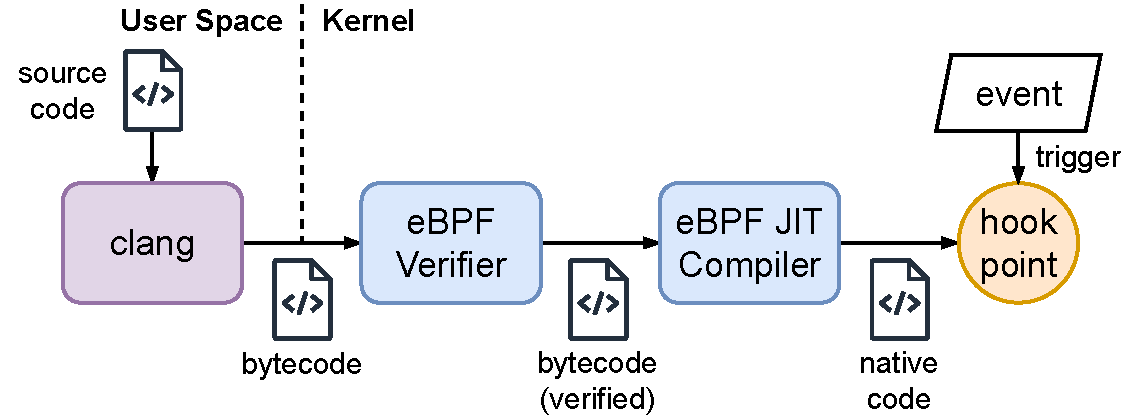
\includegraphics[width=\linewidth]{figures/sec-2-ebpf-pipeline-fig.pdf}
  \caption{The eBPF execution pipeline.}
  \label{fig:ebpf}
\end{figure}

\noindent\textbf{Source compilation.}
% \noindent\textbf{源代码编译。}
The userspace compiler does most of the pipeline's optimization.
% 用户空间编译器完成管线的大部分优化。
A language front end such as Clang lowers the source to LLVM IR, and LLVM's middle end runs its full optimization passes.
% 语言前端如 Clang 将源代码降低为 LLVM IR，LLVM 中端运行完整的优化遍。
The eBPF backend then lowers the result to bytecode restricted to the operations the instruction set defines.
% 然后 eBPF 后端将结果降低为限制在指令集定义的操作内的字节码。
Optimization research also targets this stage, where compile-time optimizers such as Merlin~\cite{mao2024merlin}, K2~\cite{xu2021synthesizing}, and EPSO~\cite{zhu2025epso} rewrite programs for speed and size.
% 优化研究也针对这个阶段，编译时优化器如 Merlin、K2 和 EPSO 重写程序以提高速度和减小大小。
The optimizers all stay within the instruction set, because the verifier rejects anything else.
% 所有优化器都停留在指令集之内，因为验证器会拒绝其他任何东西。
The instruction set has no single-instruction form for hardware idioms.
% 指令集没有硬件习语的单指令形式。
Every optimizer at this stage, including LLVM, therefore emits the idioms as multi-instruction sequences.
% 因此这个阶段的每个优化器，包括 LLVM，都将习语发射为多指令序列。

\noindent\textbf{Verification.}
% \noindent\textbf{验证。}
The verifier checks safety, changes the program little, and enforces the instruction set.
% 验证器检查安全性，对程序改动很小，并强制执行指令集。
The verifier proves memory safety, termination, and similar properties by static analysis~\cite{gershuni2019simple}.
% 验证器通过静态分析证明内存安全、终止性和类似属性。
The analysis proceeds opcode by opcode, over the 123 opcodes the instruction set defines~\cite{rfc9669}.
% 分析逐操作码进行，覆盖指令集定义的 123 个操作码。
An opcode the instruction set does not define is rejected.
% 指令集未定义的操作码会被拒绝。
The only existing way to run native code that the instruction set cannot express is to call a \emph{kfunc}, a native kernel function that a loadable module registers with BTF type metadata~\cite{kfuncs}.
% 目前运行指令集无法表达的本地代码的唯一方式是调用 kfunc，即由可加载模块使用 BTF 类型元数据注册的本地内核函数。
After a program passes, the verifier applies only a few targeted rewrites, such as dead-code elimination.
% 程序通过后，验证器只应用少量定向重写，如死代码消除。
A few systems also optimize at load time, such as KFuse~\cite{kfuse}, which merges verified programs within the instruction set.
% 少数系统也在加载时优化，如 KFuse，它在指令集内合并已验证的程序。
The verifier then passes the program to the JIT.
% 然后验证器将程序传递给 JIT。

\noindent\textbf{JIT compilation.}
% \noindent\textbf{JIT 编译。}
The kernel JIT does almost no optimization.
% 内核 JIT 几乎不做优化。
The kernel maintains one such JIT for each supported architecture.
% 内核为每个支持的架构维护一个这样的 JIT。
Translation proceeds one opcode at a time, with the eBPF registers \texttt{r0}--\texttt{r10} mapped to fixed native registers.
% 翻译逐操作码进行，eBPF 寄存器 r0--r10 映射到固定的本地寄存器。
The only optimization choices are within one instruction's encoding, such as picking the shortest immediate form on x86-64.
% 唯一的优化选择是在单条指令的编码内，如在 x86-64 上选择最短的立即数形式。
The JIT runs no general cross-instruction optimization, such as global register allocation or instruction scheduling.
% JIT 不运行通用的跨指令优化，如全局寄存器分配或指令调度。
The simple design keeps the JIT small enough to trust, a tradeoff that \S\ref{subsec:char-challenges} returns to.
% 简单的设计使 JIT 足够小、可以信任，这是一个权衡，将在后面讨论。
The multi-instruction sequences the backend emits therefore survive into the machine code unoptimized, at a cost that \S\ref{sec:characterization} measures.
% 因此后端发射的多指令序列未经优化就进入机器代码，其代价将在后面测量。